\documentclass[11pt, titlepage]{article}
%\usepackage{showframe}
\usepackage[utf8]{inputenc}
\usepackage[L7x]{fontenc}
\usepackage[lithuanian]{babel}
\usepackage{tgtermes}
\usepackage{graphicx}
\usepackage{float}
\usepackage{setspace}
\onehalfspacing


\usepackage{hyperref}
\hypersetup{colorlinks=true, linkcolor=black, filecolor=blue,
urlcolor=blue, citecolor=black}

\usepackage{caption}
\usepackage[a4paper, nomarginpar, total={175mm, 257mm},left=40mm, right=25mm, top=20mm, bottom=20mm]{geometry}


\title{Migracijos įtaka darbo rinkai}
\author{Karolina Matulevičiūtė}

\usepackage[
backend=biber,
style= apa,
url=false,
sorting=nyt
]{biblatex}
\addbibresource{references.bib}

\begin{document}
\maketitle
\tableofcontents
\newpage

\section{Įvadas}




	21 amžiuje žmonėms atsirado daugybė galimybių  ir būdų keliauti po visą pasaulį, pažinti jį, taip pat emigruoti į kitas šalis ieškant geresnio gyvenimo ir darbo.  Vieni daro tai savo noru, kiti – priversti tai daryti dėl įvairių gyvenime iškylančių situacijų. Pavyzdžiui, yra žmonių, kurie sujungia malonumą su nauda – jie išvyksta į kitą šalį studijuoti, o tuo pačiu metu ir susipažinti su pasirinktos šalies kultūra ir gyvenimo būdu. Kiti gi priversti palikti savo gimtinę dėl to, kad neranda galimybių joje pagerinti savo pačių ir savo šeimos gyvenimo sąlygas.  Tačiau nereikia pamiršti, jog bet kokia migracija turi įtakos ne tik tų žmonių, kurie migravo, tačiau ir tu žmonių, į kurių šalis yra imigruojama, ir jų gimtinių gyvenimams. Šiame darbe plačiau bus kalbama būtent apie migracijos poveikį šalies darbo rinkai. 

	Migracijos sąvoka apima bet kokį žmonių judėjimą – vienoje valstybėje ar kertant jų sienas; ilgam ar trumpam laikotarpiui; savanorišką ar priverstinę; ieškant kitos darbo ar bedarbystės vietos; legalią ar nelegalią; migraciją siekiant pakeisti politinę, socialinę, ekonominę, kultūrinę ar kitokią aplinką. Iš šito apibrėžimo matome, jog migracija yra išskiriama pagal vietą, laiką, judėjimo priežastys ir t.t. Nuo migracijos reiškinio vertinimo ir migracijos aiškinimo priklauso ir konkrečios valstybės taikomų priemonių pasirinkimas (Vepšta P. ir kt., 2009). Asta Stulgienė ir Asta Daunorienė savo darbe ,,Migracijos poveikis darbo jėgos rinkos pusiausvyrai“ kalba apie tai, kad migracija yra dinamiškas ir įvairialypis procesas, susijęs su šalių sąlygomis, jų traukos ir stūmos jėgomis, veikiantis socialinę, ekonominę, politinę, demografinę, ir kitas šalių sistemas, įtakojantis jų gerovę bei vystymąsi. 

	Migracijos procesai daugiau mokslininkų dėmesio sulaukė dar XIX a. antroje pusėje. Lietuvos priklausimo TSRS laikais domėjimasis migracija buvo laikomas tabu. Tačiau Lietuvai atgavus nepriklausomybę 1990 m. migracijos procesų aktualumas pradėjo augti. 

\section{Darbo jėgos migracijos priežastys ir pasekmės}

	Migracijos režimas Europos sąjungoje remiasi laisvu asmenų ir darbo resursų judėjimu. 1990- tų metų pradžioje darbo migracija iš Centrinių ir Rytinių Europos šalių vis dar buvo ribojama laikino darbo užimtumo programomis, tačiau kartu su vizinio režimo liberalizacija ir augančia darbo jėgos paklausa ES šalyse laikui einant ji įgavo gana rimtą mastą. Didžiausias gyventojų skaičiaus sumažėjimas dėl emigracijos per paskutinius dvidešimt metų buvo registruojamas Baltijos šalyse, Bulgarijoje ir Rumunijoje. 
	
	Algis Junevičius „Laisvas darbo jėgos...“ teigia: „Europos darbo rinką sudaro trys kategorijos samdomų darbuotojų. Pirmoji – pati gausiausia – valstybių narių darbuotojai, kurie dirba savo šalies teritorijoje. Antrąją kategoriją sudaro migrantai ES piliečiai, turintys tas pačias teises kaip ir nacionaliniai darbuotojai.... Trečiajai samdomų darbuotojų kategorijai priklauso darbuotojai, atvykę iš trečiųjų šalių. Jeigu jie dirba legaliai, jų teisės įvažiuojant į šalį ir įsidarbinant yra ribojamos.“ Svarbu aptarti priežastys, kurios skatina žmones emigruoti. 
	
	Darbo jėgos migraciją pirmiausia sukelia ekonominės priežastys, tarp kurių ryškiausios yra nedarbas ir pajamų bei gyvenimo lygio skirtumas (Filer ir kt., 1996; Ehrenberg, ir kt., 1997). Didelis nedarbas, santykinai mažas darbo užmokestis , prastos darbo sąlygos šalyje verčia darbuotoją ieškoti darbo kitur \parencite{stulgiene2009migracijos}. Svarbiausi stimulai yra – galimybė gauti didesnį atlyginimą arba pajamas, nedidelis geografinis atstumas (tačiau daugeliui ir tai tampa ne taip svarbu), geresnė padėtis darbo rinkoje, politinės ar tautinės problemos gimtinėje. Pajamų skirtumas tarp šalių ir yra svarbiausia migraciją sąlygojanti priežastis.  Jeigu žmogus supranta, jog jo netenkina tas gyvenimo lygis ir sąlygos, kurias jis gauna savo šalyje, ir žino, jog gali tai pagerinti kitoje, tai yra didelė tikimybė, jog žmogus pasirinks geresni sau varianta. Ir tai yra labai natūralu ir normalu. 2018 metais emigravo 32,2 tūkstančio Lietuvos gyventojų. Didžioji dauguma išvykstančių iš Lietuvos yra darbo migrantai.
	
\begin{figure}[H]
\center	
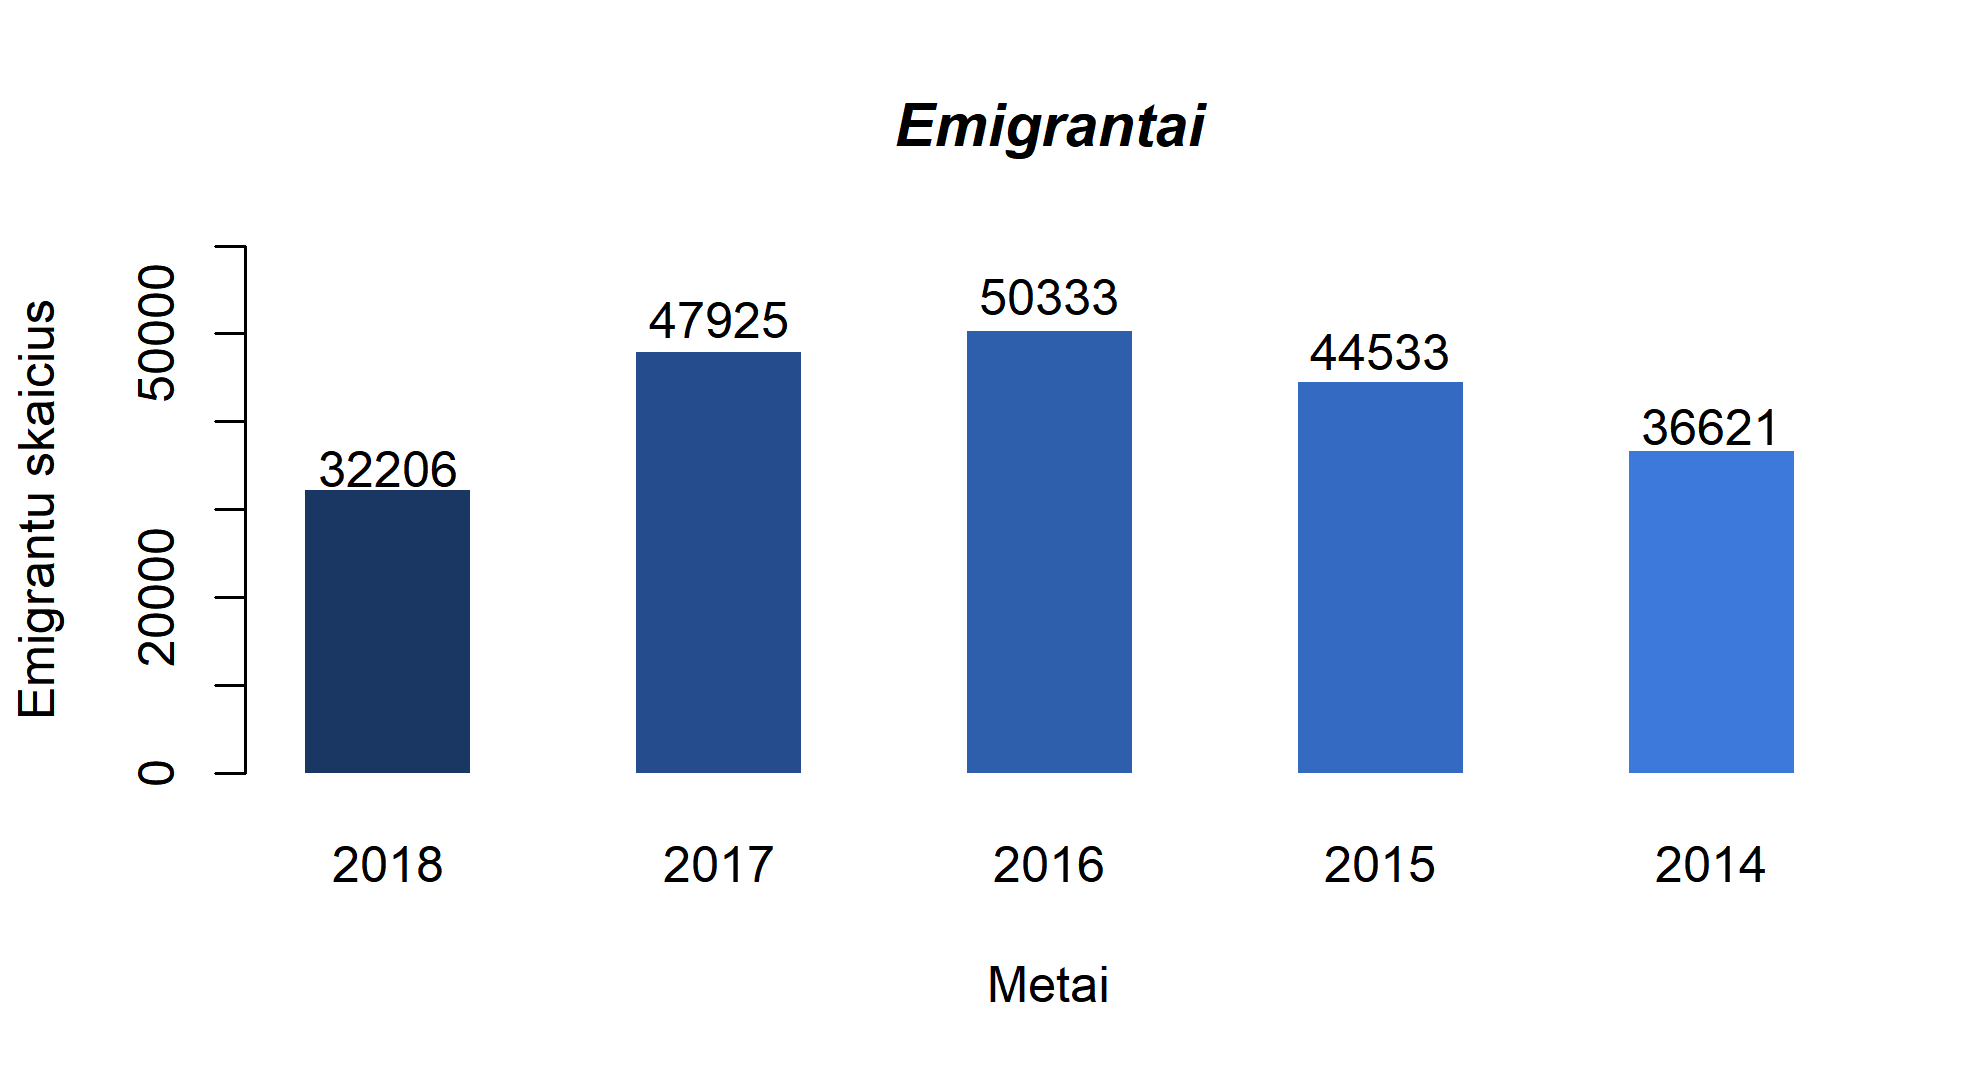
\includegraphics[scale=0.85]{emigrantai}	
\caption{Iš Lietuvos emigravusiųjų skaičius}
\end{figure}
	
	Jeigu tarp dviejų šalių nėra jokių kliūčių ir migracija vyksta laisvai, tai iš šalies, kur darbo užmokestis mažesnis, išvažiuojant asmenims, dėl to, kad darbo pasiūla mažės, darbo užmokestis didės, o šalyje, į kurią yra imigruojama, darbo užmokestis mažės dėl to, kad darbo pasiūla didės. Laikui einant, darbo užmokestis abejose šalyse keisis ir susilygins ir nedarbas neatsiras. Tačiau darbo jėgos migracija ne visada lygina užmokestį. Pavyzdžiui, mažiau ekonomiškais išsivysčiusiose šalyse aukštos kvalifikacijos žmonės gauna atlyginimą, kuris yra mažesnis už jų ribinį produktą, todėl dėl jų emigracijos pasiliekančiųjų šalyje vidutinis darbo užmokestis mažėja \parencite{matiuvsaityte2003darbo}. 
	
	Sprendimą migruoti veikia įvairūs veiksniai, kurių vertė kiekvienam individui yra skirtinga ir kinta laike. Teoriškai asmuo emigruos, jei nauda iš to viršys kaštus. Žmonės emigruoja manydami ir tikėdamiesi, kad tai pakeis jų gyvenimą geresne linkme, kad jie galės sutekti savo šeimai – dažniausiai likusiai gimtinėje – geresnes gyvenimo sąlygas. Paprastai sakant žmogus palygina savo gyvenamosios vietos trūkumus su vietos, į kurią jis nori emigruoti, pranašumais. „Stūmos ir traukos veiksniai reiškiasi kaip įvairūs ekonominiai (atlyginimų dydis, ekonominis ne/augimas, nedarbas), socialiniai-kultūriniai (migracijos „mada“, tradicijos, ne/tolerancija), politiniai (politinė santvarka, rinkimų rezultatai), psichologiniai (gebėjimas priimti asmeninius sprendimus), saugumo (dėl karinių ar kitų konfliktų, politinių ar kitų represijų), geografiniai (klimato sąlygos), populiacijos/demografiniai ir kiti veiksniai.“ \parencite{damuliene2013migracijos}.

\section{Migracijos poveikis darbo rinkai}

	Dažniausiai yra prognozuojamas neigiamas darbuotojų migracijos poveikis ES valstybių darbo rinkoms. Reikia atkreipti dėmesį į tai, kad atkeliaujanti iš Rytų ir Vidurio Europos šalių darbo jėga yra pigesnė negu ekonomiškai išsivysčiusiose šalyse. Dėl šitos priežasties darbo jėgos kaina gali mažėti, o dėl to didės nedarbas, kuris ir taip yra problema Europoje.
	
	Darbo jėgos trūkumas yra auganti našta Lietuvos ekonomikai. Įmonės, norėdamos kompensuoti senų darbuotojų paradimą, bando įdarbinti naujus darbuotojus, tačiau bet kokia personalo kaita reikalauja papildomų sąnaudų ir pereinamojo laikotarpio, kuris yra reikalingas tam, kad įmonė galėtų rasti tinkamos kvalifikacijos darbuotojus arba sutekti tinkamą kvalifikaciją savarankiškai, jos pačios imasi mokyti naujus darbuotojus \parencite{januvsauskas2009vsiuolaikiniai}.
	
	Migracija darbo rinkai daro įtaką dvejopai: pirma – keisdama Lietuvos gyventojų, taip pat bedarbių, užimtųjų darbo jėgos skaičių: antra – emigrantų pinigų pervedimais sąlygodama vartojimą ir ekonomikos augimą.
Vepšta Povilas ir kiti darbo autoriai teigia, jog darbo jėgos trūkumą gali kompensuoti: 
-	investicijos į esančius darbuotojus keliant jų našumą;
-	investicijos į technologijas, kurios leistų sumažinti reikalingų darbuotojų skaičių;
-	papildomos darbo jėgos pritrukimas į darbo rinką, pavyzdžiui, imigrantų iš kitų valstybių ar iš neaktyvios darbo jėgos Lietuvoje.
	
	Kalbant apie neaktyvius gyventojus galima kreiptis į \href{https://osp.stat.gov.lt/statistiniu-rodikliu-analize#/} {Lietuvos statistikos departamentą} kiek būtent jų buvo. 2018 metais darbingo amžiaus neaktyvių gyventojų skaičius svyravo 407-435 tūkst., palyginus su 2019 metų pirmu ketvirčiu ir 2017 metais, matome, jo kasmet skaičius mažėja. Tai reiškia, kad vis daugiau žmonių yra įtraukti į valstybės gyvenimą.

\begin{figure}[H]
\center
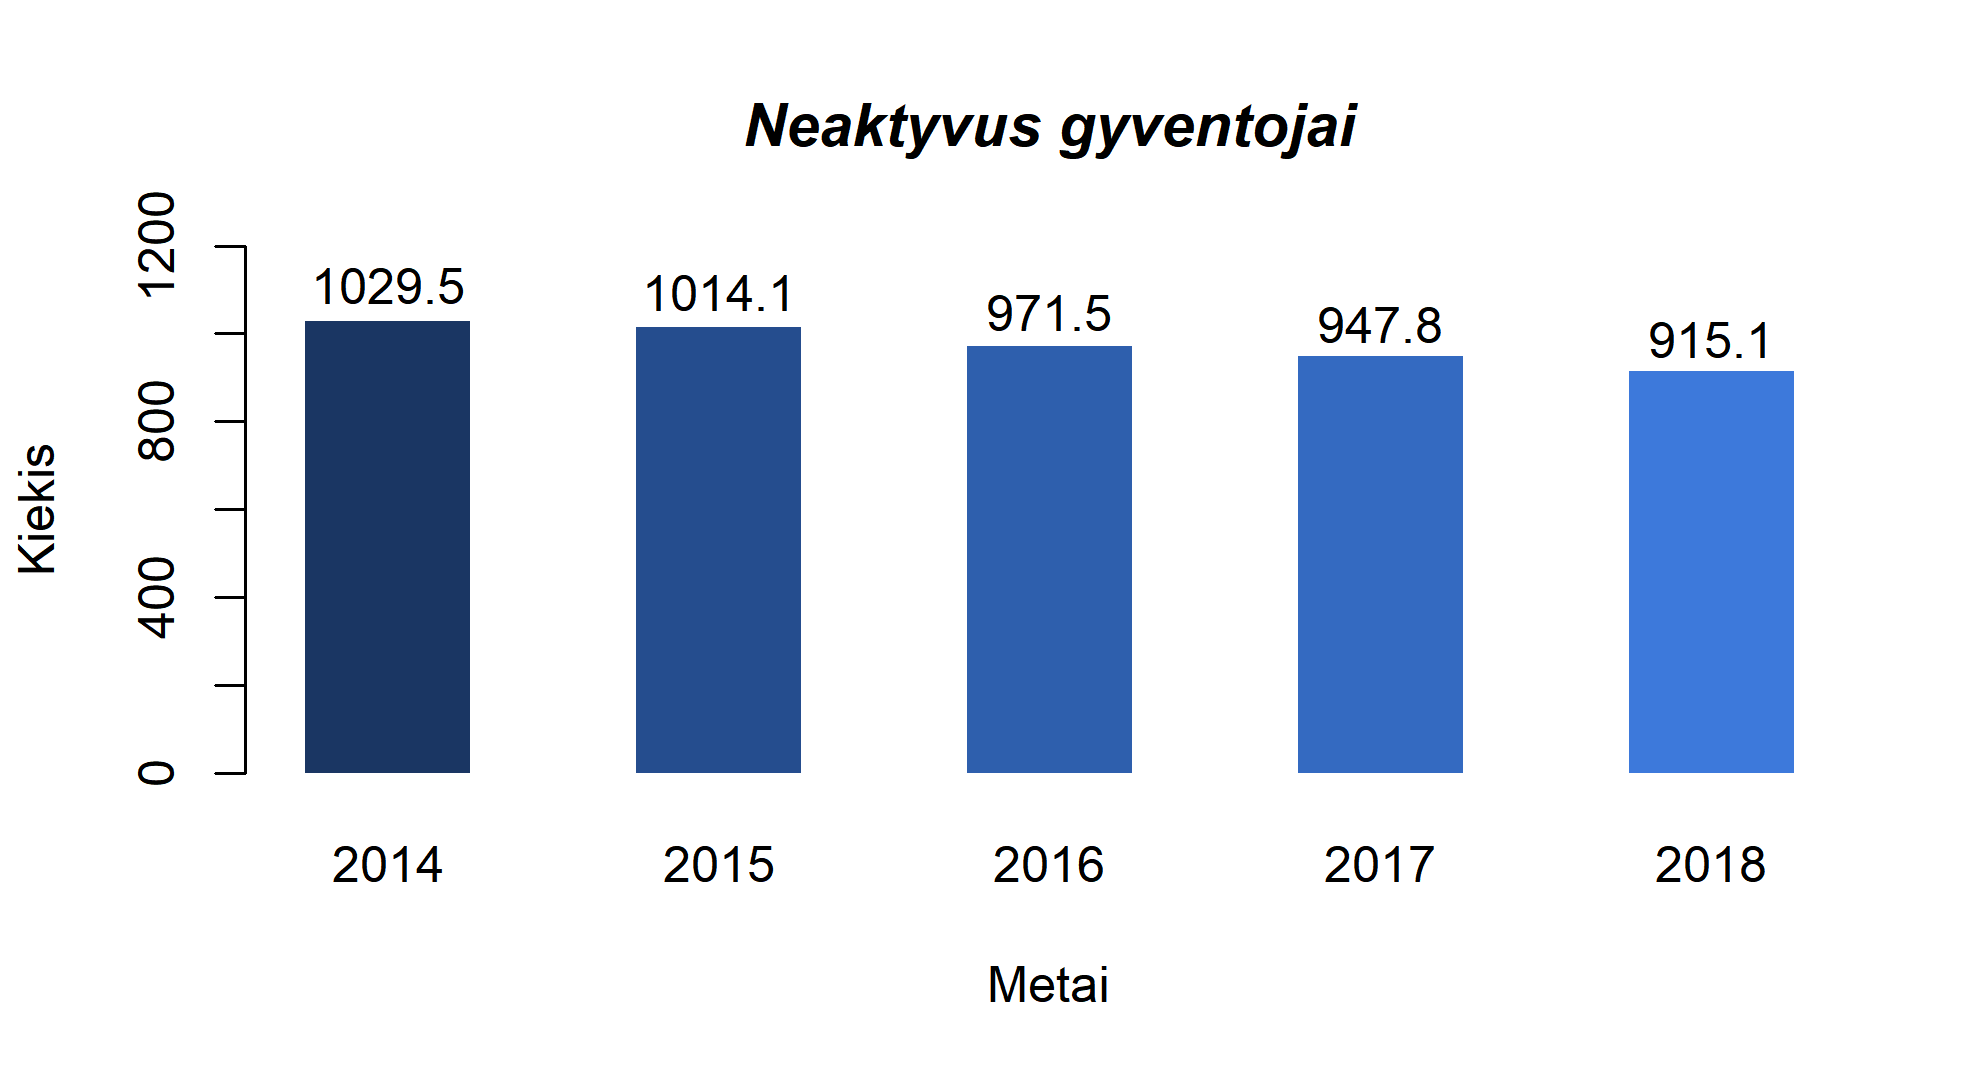
\includegraphics[scale=0.85]{neaktyvus}
\caption{Neaktyvių Lietuvos gyventojų skaičius}
\end{figure}

	
	
	Tarptautinė migracija gali būti trumpalaikė ir ilgalaikė. Manoma, jos ilgalaikė migracija yra žalingesnė, nes didžioji dalis išvykusiųjų nebegrįžta į gimtinę, prarandamos lėšos, kurios buvo investuotos į žmogaus išsilavinimą, prarandamas specialistas. Tuo tarpu trumpalaikę emigraciją galima vertinti kaip išsigelbėjimą sunkiu ekonominiu laikotarpiu, nes sumažėja nedarbas, padidėja žmonių pajamos, svetur įgyjama naudingos patirties \parencite{damuliene2013migracijos}.
	
	Pagrindinė problema, su kuria susiduria darbuotojai, atvykstantys ne iš ES šalių yra administraciniai apribojimai. Lietuva mielai priima ES valstybių narių piliečius ir taiko tokias pat taisykles įdarbinant kaip ir Lietuvos piliečiams. Tačiau taiko griežtas procedūras darbuotojams iš trečiųjų šalių. Nepaisant to, darbdaviai su didesniu noru priimtų tokius darbuotojus dėl to, kad tie sutiktų dirbti už mažesnį atlyginimą negu pareikalautų vietiniai gyventojai arba ES šalių piliečiai. Tai sukelia problemų vietinių gyventojų įsidarbinimui. Vis dažniau girdima žmonių nuomonė apie tai, kad kitataučiai yra viena iš priežasčių, kuri stipriai paveikia mūsų šalies darbo rinką, sumažina darbo jėgos vertę,  ,,numuša“ atlyginimus ir trukdo vietiniams gyventojams, kurie gyvena Lietuvoje nuo pat gimimo arba keliasdešimt metų, įsidarbinti. Todėl nenuostabu, kad kartais visuomenės nuomonė yra nepalanki į plėtrą, o ypač į laisvo (ar su nedidelėmis kliūtimis) darbuotojų judėjimo principą. Lietuvos darbo rinka yra labai patraukli kaimyninių šalių darbuotojams – baltarusiams, ukrainiečiams ir rusams. To priežastis yra kelis kartus didesni atlyginimai. Pavyzdžiui Lietuvoje vidutinis bruto darbo užmokestis šiuo metu yra 1262,7 Eur, tuo tarpu kaimynėje Baltarusijoje tik 414,6 Eur, o Rusijoje – 488,6 Eur. Iš šito matome, jog vidutinis atlyginimas Lietuvoje yra maždaug 3 kartus didesnis.
	

	Vepšta Povilas ir kiti darbo „Šiuolaikiniai migracijos procesai...“ autoriai teigia: „Esant dabartinei ekonominei situacijai ir egzistuojančiam teisiniam imigracijos proceso reglamentavimui, Lietuva kol kas yra pajėgi konkuruoti su kaimyninėmis valstybėmis dėl darbo jėgos imigracijos iš trečiųjų šalių, tačiau atsižvelgiant į vieną iš žemiausių darbo užmokesčių lygių ES Lietuvai sunku konkuruoti su daugeliu ES valstybių narių.“ Dėl šitos priežasties Lietuvai, pasitelkus trūkstamą aukštos kvalifikacijos darbo jėgą iš trečiųjų šalių, yra svarbiausia plėtoti ūkio sektorius, kuriuose yra sukuriama didžiausia pridėtinė vertė ir kurie gali turėti įtakos Lietuvos ekonomikos augimui  bei didintų jos konkurencingumą. Tokiu būdu bus bandoma užtikrinti darbo užmokesčio augimą Lietuvoje ir jo galimybes konkuruoti su kitomis ES valstybėmis narėmis. 

\section{Išvados}

	Migracijos tema šiuolaikiniame pasaulyje yra labai svarbi ir aktuali. Kadangi bet koks žmonių judėjimas daro didžiulę įtaką šalių ekonomikai, o būtent darbo rinkai.


\begin{enumerate}
\item Svarbiausia priežastis dėl kurios žmones pasiryžta migruoti yra finansinė. Žmonės įvertina savo gyvenimo lygį ir susimąsto, ar galėtų tai pakeisti. Jeigu kitoje vietoje žmogus gali pagerinti savo gyvenimą ir gyventi geriau ir sočiau, tai, žinoma, jis pasirinks geresnį būdą.
\item Žmogus visada pasirinks migraciją, jeigu teikiama nauda bus didesnė už kaštus. Sprendimą migruoti veikia įvairūs veiksniai, kurių vertė kiekvienam individui yra skirtinga ir kinta laike.
\item Tyrinėtojų prognozės dėl migracijos dažniausiai yra neigiamos. Yra manoma, jog migrantai iš ekonomiškai silpnesnių ir mažiau išsivysčiusių šalių sutinka dirbti už mažesnį atlyginimą ir dėl to mažina darbo jėgos vertę labiau išsivysčiusiose šalyse.
\item Darbo jėgos trūkumo problema Lietuvoje vis didėja. Įmonės priverstos pačios apmokinti savo darbuotojus arba ieškoti naujų kvalifikuotų darbuotojų. Ir pirmas ir antras variantas užima laiką ir atneša didesnes sąnaudas įmonėms. 
\item Tarptautinė migracija yra klasifikuojama kaip ilgalaikė ir trumpalaikė. Pirmoji yra laikoma teigiama, nes padidėja pajamo, mažėja nedarbas ir t.t, o ilgalaikė – neigiama, nes valstybės patiria išlaidas ir netenka darbuotojų.

\end{enumerate}

\newpage
\nocite{*}
\printbibliography[title= Literatūros sąrašas]



\end{document}